\chapter{Setup sperimentale}

Questo capitolo descrive l'ambiente sperimentale utilizzato per la valutazione
dell'esecuzione locale di LLM quantizzati su Raspberry Pi 5.

Le metriche di analisi adottate nel dettaglio e le procedure sperimentali per
l'esecuzione dei benchmark vengono descritte nel capitolo successivo a questo.

\section{Configurazione hardware}

Oltre al Raspberry Pi 5 e al computer host per le misurazioni, vediamo gli accessori
hardware fondamentali da tenere conto.

\subsection{Alimentazione e misura del consumo tramite il PMIC}
\label{sec:pmic}
Il monitoraggio del consumo energetico del sistema è stato effettuato sfruttando
direttamente il \textit{PMIC} (\textit{Power Management Integrated Circuit}) di
cui è dotato il Raspberry Pi 5. Il PMIC è il circuito integrato che genera e
regola le diverse tensioni di alimentazione della scheda (per il SoC, la memoria,
i sottosistemi di I/O e così via) a partire dai 5~V forniti in ingresso. Oltre a
questa funzione, il PMIC del Pi 5 integra un convertitore analogico-digitale
(\textit{ADC}) che misura tensione e corrente su dodici distinti rami di
alimentazione della scheda.

Tali grandezze sono accessibili via software attraverso l'utility di sistema
\texttt{vcgencmd}: il comando \texttt{vcgencmd pmic\_read\_adc} restituisce, per
ciascun ramo, la corrente e la tensione istantanee. La potenza istantanea
assorbita dalla scheda viene stimata sommando i contributi dei dodici rami, come
descritto nel dettaglio nel capitolo successivo. Questo approccio consente di
misurare il consumo del Raspberry Pi 5 \emph{senza alcun hardware di misura
esterno}, utilizzando i sensori già integrati sulla scheda; la metodologia
adottata riprende quella del progetto open source
\textit{RPi5-power}~\cite{jfikar_rpi5power}. Tale progetto propone anche una
correzione empirica per stimare il consumo reale alla presa, che però è tarata su
una singola scheda e non trasferibile ad altre unità; in questo lavoro si registra
quindi direttamente la somma non corretta delle potenze dei rami, misura coerente
e adeguata al confronto tra modelli (v.\ Capitolo successivo).

Per l'alimentazione è stato impiegato l'\textbf{alimentatore ufficiale del
Raspberry Pi 5} (USB-C, 5,1~V, fino a 3~A, 15~W), collegato alla porta di
alimentazione \textit{USB-C} della scheda. L'impiego dell'alimentatore ufficiale,
progettato per il Pi 5, garantisce una tensione stabile ed evita condizioni di
sottoalimentazione (\textit{undervoltage}) durante i picchi di assorbimento in
carico. Si è scelto deliberatamente di \emph{non} alimentare il dispositivo
tramite i pin GPIO: tale modalità bypassa le protezioni dell'ingresso USB-C ed
espone il PMIC al rischio di danneggiamento~\cite{raspberrypi_gpio}. Misurando il
consumo direttamente dal PMIC, non è inoltre necessario interporre alcuno
strumento sulla linea di alimentazione.

\subsection{Ventola di raffreddamento}
Il Raspberry Pi 5 è dotato di una \textit{ventola di raffreddamento attiva},
integrata nel case utilizzato per gli esperimenti e alimentata tramite il
connettore a quattro pin contrassegnato dalla dicitura ``FAN'' sulla scheda.
La presenza del sistema di raffreddamento consente di mantenere la temperatura
operativa del dispositivo entro valori adeguati durante l'esecuzione di carichi
computazionali intensivi.

\subsection{Connessione via Ethernet}

Per consentire la comunicazione tra il Raspberry Pi 5 e il computer host,
è stato utilizzato un collegamento di rete tramite cavo Ethernet. Tale
configurazione permette di accedere al dispositivo mediante protocollo \textit{SSH},
consentendo l'esecuzione remota dei comandi e delle inferenze LLM.\@

Per semplificare l'accesso remoto, il Raspberry Pi 5 è stato configurato con un
indirizzo \textit{IP statico}. A differenza di una configurazione basata su protocollo
\textit{DHCP}, che può assegnare un indirizzo IP differente a ogni connessione,
questa soluzione garantisce che il dispositivo sia sempre raggiungibile allo stesso
indirizzo, rendendo più affidabile l'automazione degli esperimenti e l'esecuzione degli
script di acquisizione.

La scelta di una connessione cablata è inoltre motivata dalla necessità di
garantire condizioni sperimentali il più possibile controllate e riproducibili.
Rispetto a una connessione Wi-Fi, il collegamento Ethernet presenta infatti un
comportamento più stabile e prevedibile, riducendo la variabilità del carico di
rete e del consumo energetico dovuta a interferenze, fluttuazioni del segnale o
ad altre attività del sottosistema wireless. In questo modo è possibile ottenere
una stima più accurata del consumo energetico attribuibile esclusivamente
all'esecuzione dei modelli quantizzati.

La maggiore stabilità del consumo del sistema in condizioni di inattività
(\textit{idle}) consente inoltre di utilizzare tale valore come riferimento per
stimare con maggiore accuratezza il consumo energetico aggiuntivo introdotto dal
processo di inferenza, riducendo l'influenza di fattori esterni non direttamente
correlati all'esecuzione dei modelli.

\section{Configurazione software}

\subsection{Software del Raspberry Pi 5}

Sul Raspberry Pi 5 è stato installato il sistema operativo \textbf{Raspberry Pi OS (64-bit)}
su una scheda microSD da 32 GB, utilizzata come memoria di archiviazione principale.
Durante la fase di avvio, il sistema operativo viene caricato dalla microSD, fornendo
l'ambiente software necessario per l'esecuzione dei sei modelli quantizzati discussi
nel Capitolo 1.

Per l'inferenza dei modelli è stato adottato il framework \textbf{\texttt{llama.cpp}},
progettato per consentire l'esecuzione efficiente di Large Language Models anche su dispositivi
caratterizzati da risorse computazionali limitate. La scelta di questo framework è motivata
dalla possibilità di eseguire modelli quantizzati in modo ottimizzato, configurare il numero
di thread impiegati durante l'inferenza e gestire l'esecuzione tramite interfaccia a riga di comando.
Inoltre, rispetto ad altri framework esistenti, offre una maggiore flessibilità nella selezione dei modelli
quantizzati supportati.

\subsection{Software del computer host}

Sul computer host, con sistema operativo Windows 11 (64-bit, Intel), è stato
sviluppato uno script in linguaggio \textbf{Python} che automatizza l'intera
procedura sperimentale. Poiché il consumo viene misurato direttamente dal PMIC
del Raspberry Pi 5, non è richiesto alcun software di controllo di strumenti di
misura esterni: il computer host coordina l'esperimento comunicando con il Pi
esclusivamente via \textit{SSH} sul collegamento Ethernet.

La comunicazione con il Raspberry Pi 5 avviene tramite la libreria Python
\texttt{Paramiko}, che consente sia di pilotare l'inferenza dei modelli
(avvio di \texttt{llama.cpp}, invio dei prompt) sia di leggere periodicamente il
PMIC eseguendo da remoto il comando \texttt{vcgencmd pmic\_read\_adc}. In
particolare, lo script esegue le seguenti operazioni:
\begin{itemize}
    \item connessione via SSH al Raspberry Pi 5 e impostazione dei parametri di
        acquisizione (cadenza di campionamento del PMIC);
    \item campionamento del consumo dal PMIC e delimitazione delle finestre di
        misura relative a ciascuna inferenza;
    \item esecuzione automatica dell'inferenza dei modelli quantizzati;
    \item acquisizione e memorizzazione dei dati sperimentali;
    \item elaborazione delle misure raccolte per il calcolo delle metriche relative
        al consumo energetico, alle prestazioni e alla qualità delle risposte;
    \item generazione automatica dei grafici impiegati nell'analisi comparativa dei risultati sperimentali.
\end{itemize}

Lo script viene eseguito sul computer host all'interno di un ambiente virtuale Python
isolato (\texttt{venv}), nel quale le dipendenze necessarie sono installate a versioni
fissate tramite il file \texttt{requirements.txt}.\footnote{Le dipendenze possono essere
installate con il comando \texttt{pip install -r requirements.txt}.} L'adozione di un
ambiente isolato con dipendenze versionate contribuisce alla riproducibilità
dell'esperimento.

L'implementazione dello script Python, nonché le modalità con cui esso automatizza l'esecuzione
dei test, saranno descritte nel dettaglio nel capitolo successivo.

L'architettura \textit{hardware} finale del sistema di acquisizione automatizzato è illustrata
in Figura~\ref{fig:hw_architecture}.

\begin{figure}[htbp]
    \centering
    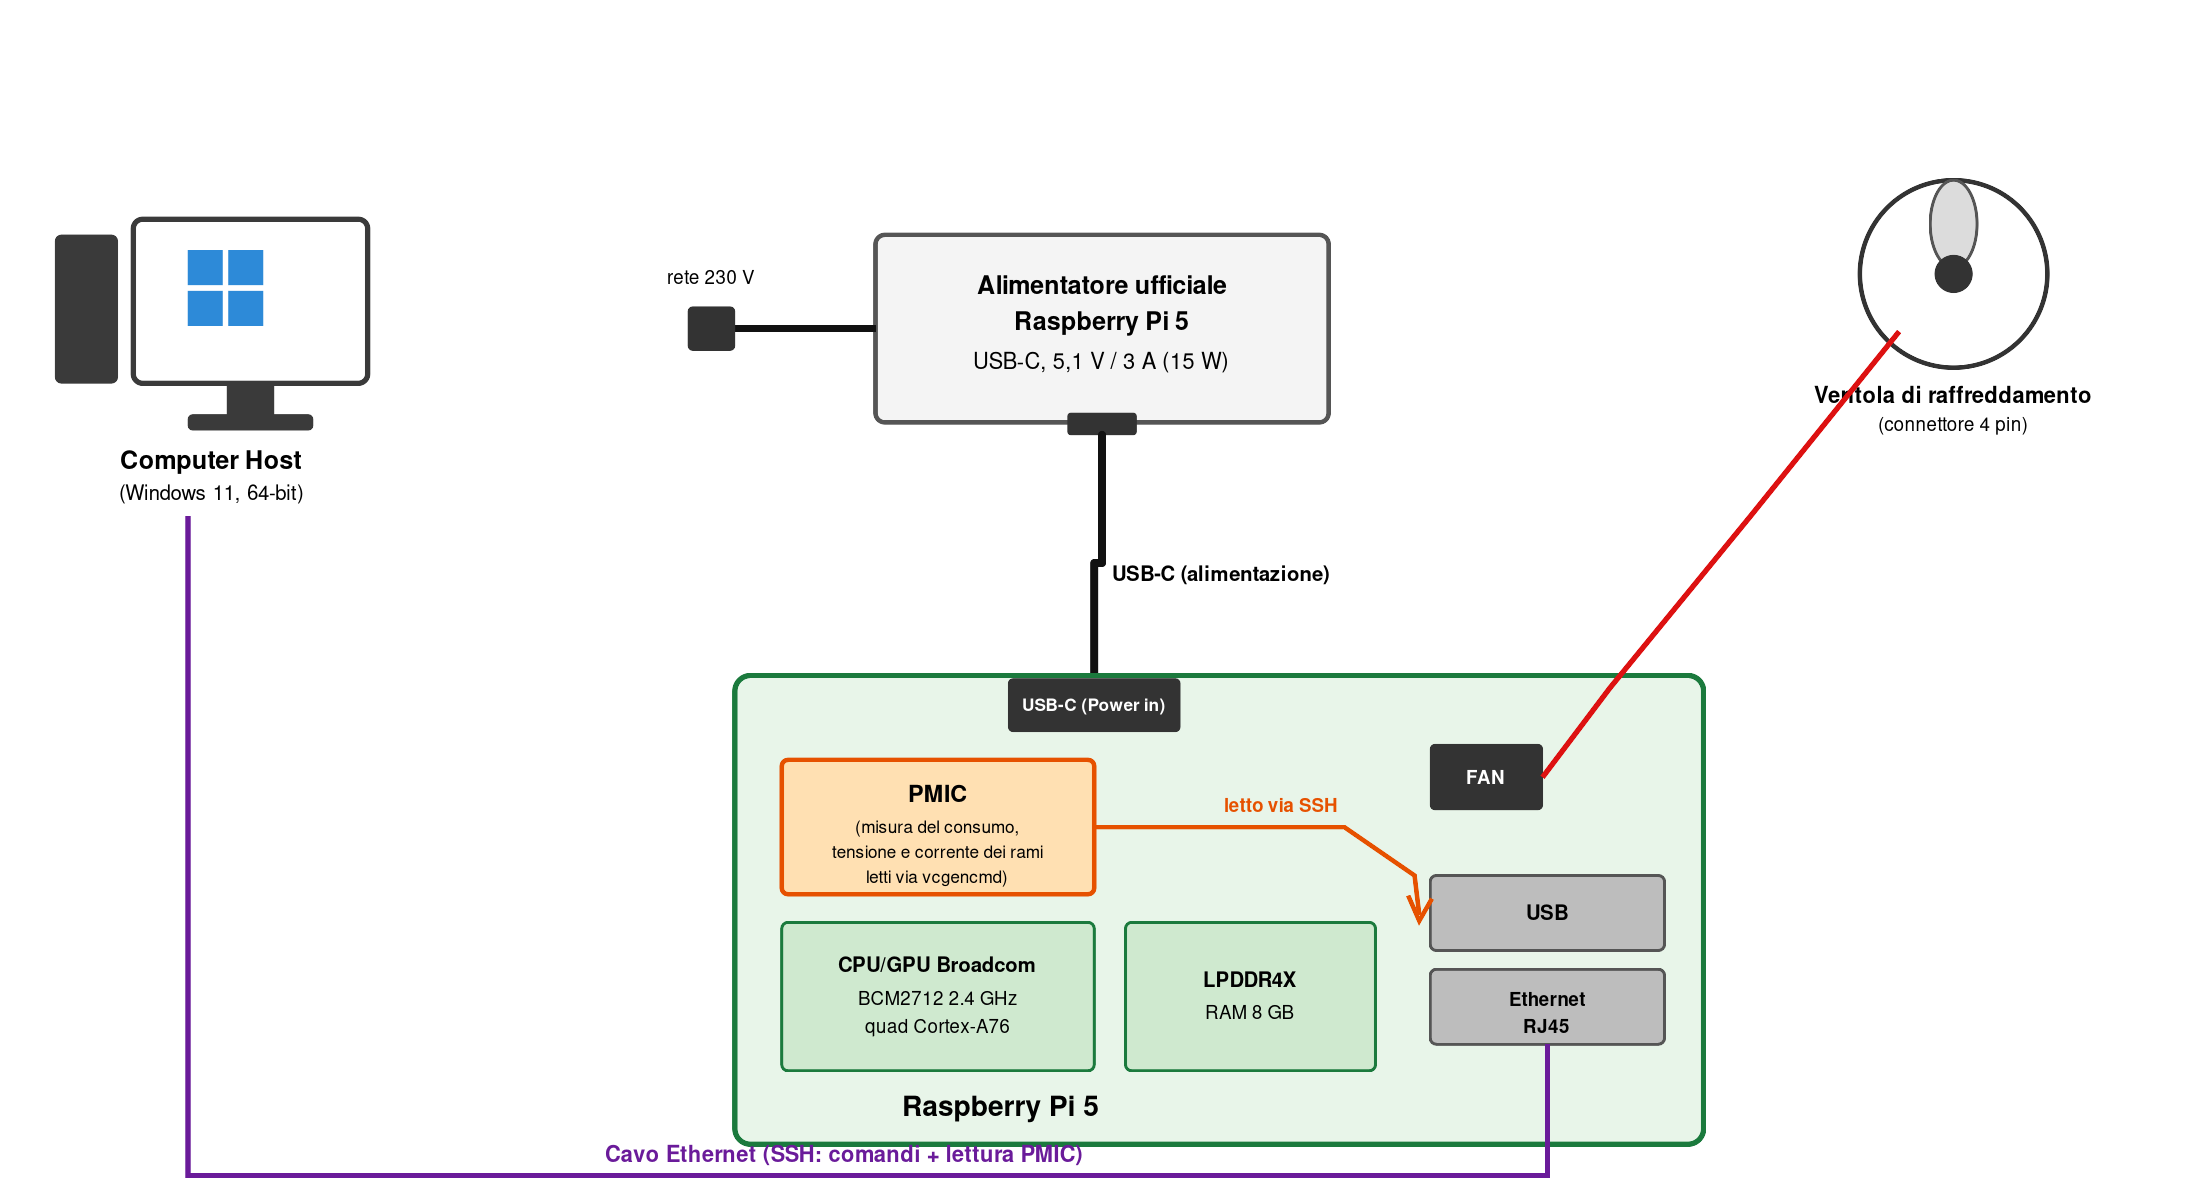
\includegraphics[width=\textwidth]{./imm/hw_architecture.png}
    \caption{Architettura hardware del sistema di acquisizione automatizzato.}
    \label{fig:hw_architecture}
\end{figure}

L'architettura \textit{software} finale del sistema di acquisizione automatizzato è illustrata
in Figura~\ref{fig:sw_architecture}.

\begin{figure}[htbp]
    \centering
    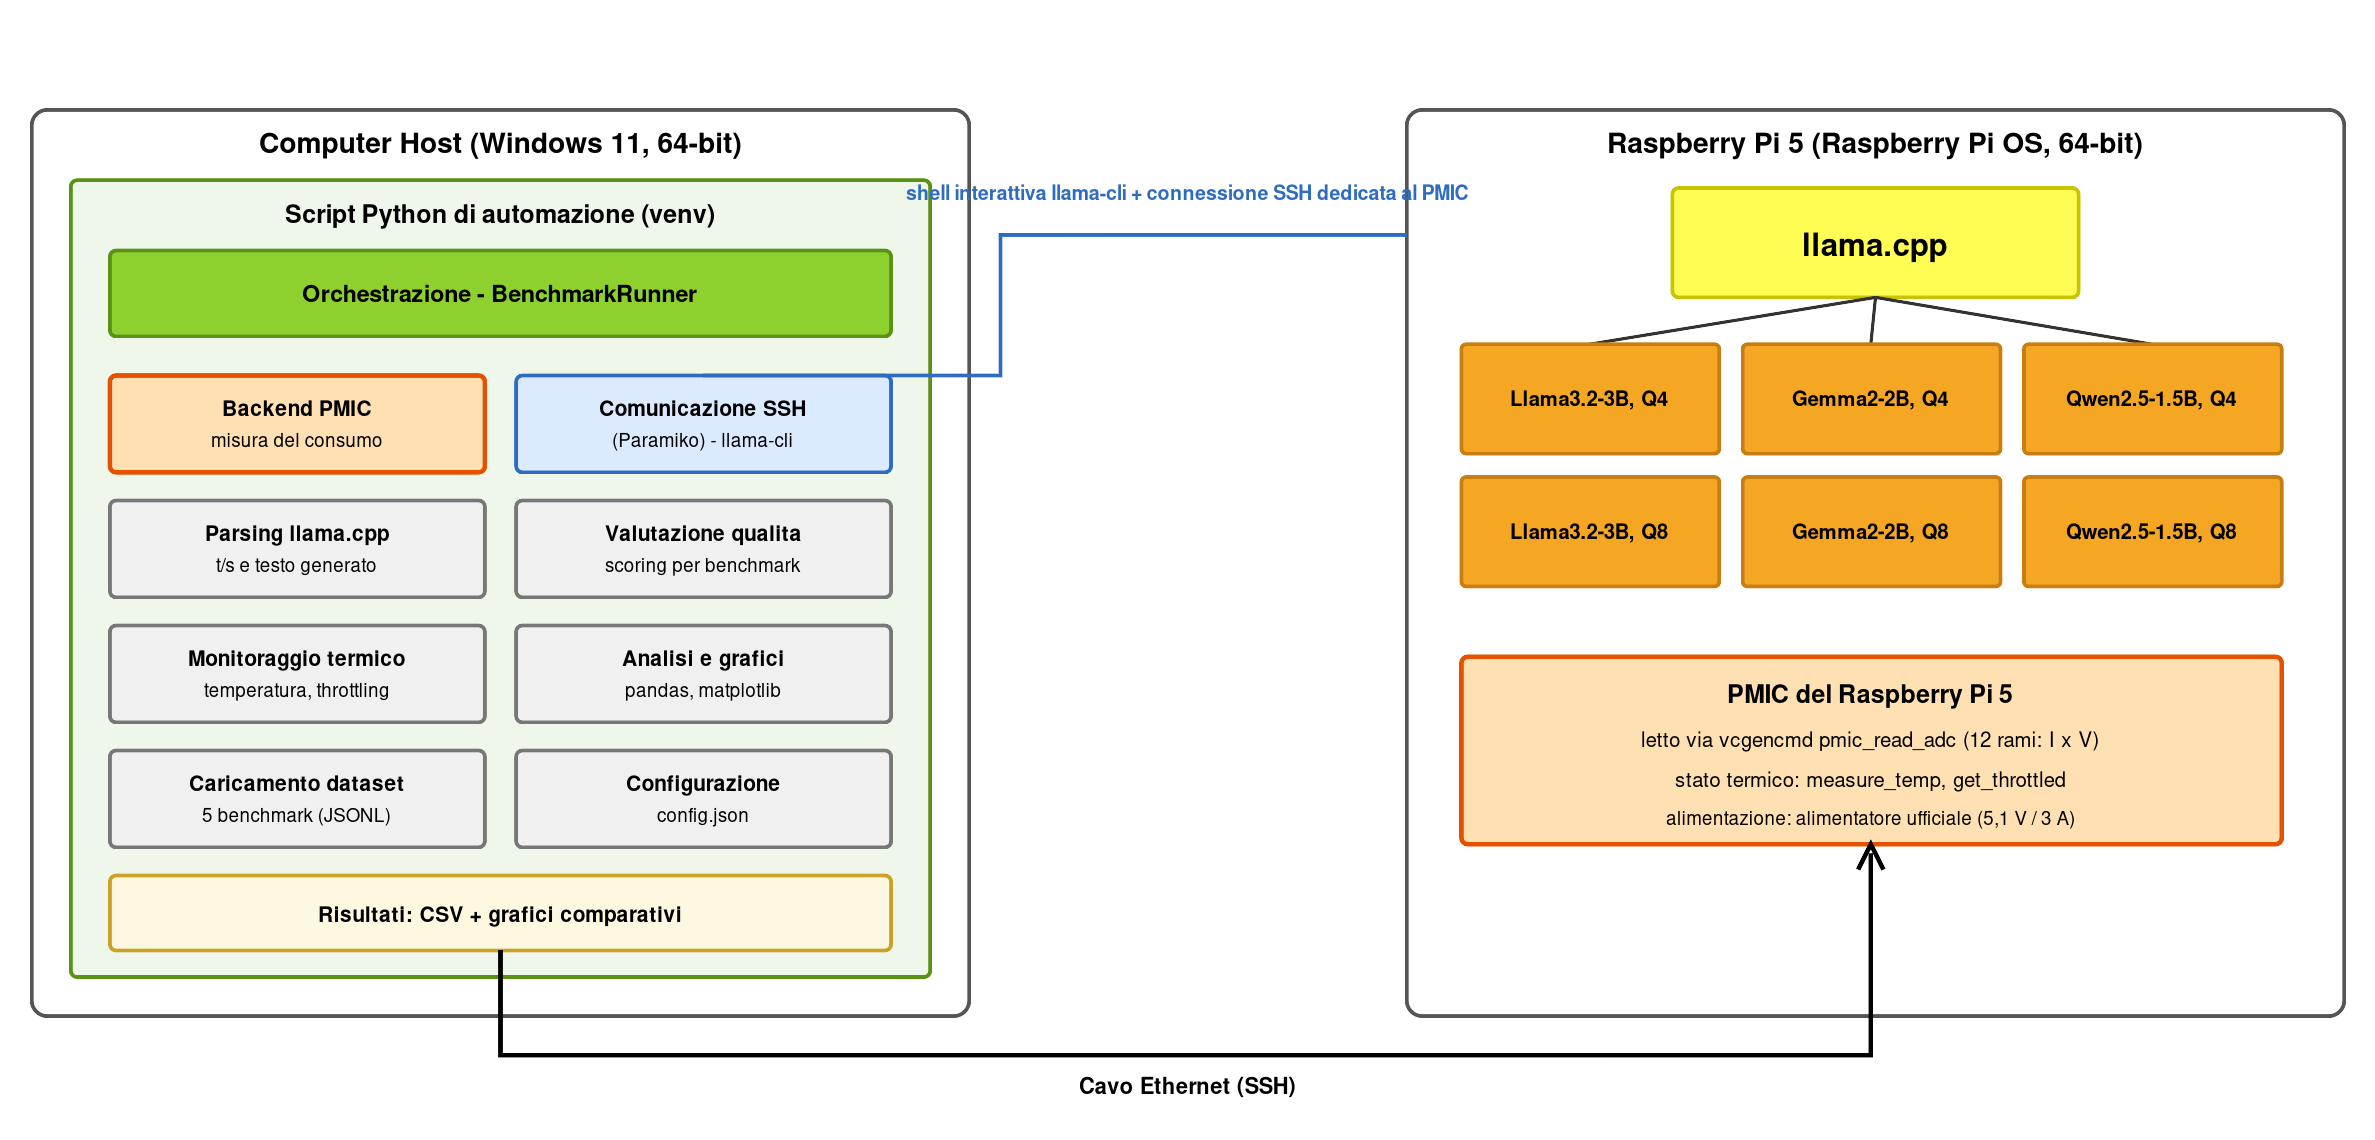
\includegraphics[width=\textwidth]{./imm/sw_architecture.png}
    \caption{Architettura software del sistema di acquisizione automatizzato.}
    \label{fig:sw_architecture}
\end{figure}
